\documentclass[border=6pt]{standalone}
\usepackage{tikz}
\usepackage{fontspec}
\setmainfont{Times New Roman}  % journal rule: figure text in Times New Roman
\usetikzlibrary{arrows.meta,positioning,shapes.geometric,fit,backgrounds,calc}
\begin{document}
\resizebox{16.2cm}{!}{%
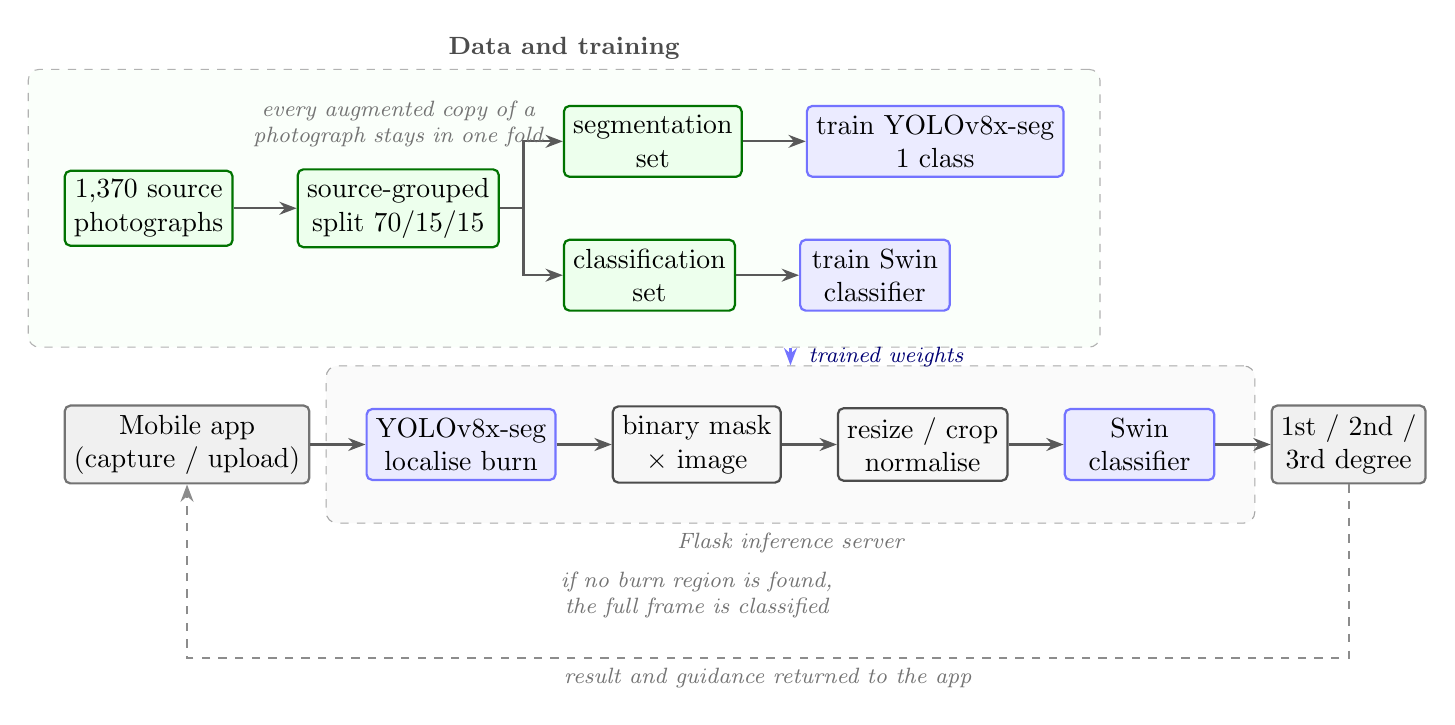
\begin{tikzpicture}[
  font=\normalsize,
  >={Stealth[length=2.2mm]},
  box/.style={rectangle, rounded corners=2pt, draw=black!70, thick, align=center,
              minimum height=9mm, minimum width=19mm, fill=black!3},
  model/.style={box, fill=blue!8, draw=blue!55},
  io/.style={box, fill=black!6, draw=black!55},
  data/.style={box, fill=green!7, draw=green!45!black},
  lab/.style={font=\footnotesize\itshape, text=black!55},
  hdr/.style={font=\small\bfseries, text=black!70},
  arr/.style={->, thick, draw=black!65},
  wts/.style={->, thick, dashed, draw=blue!55},
]

% ---------------------------------------------------------------- training row
\node[data] (src) {1{,}370 source\\photographs};
\node[data, right=8mm of src] (split) {source-grouped\\split 70/15/15};
\node[data, right=8mm of split, yshift=8.5mm] (segset) {segmentation\\set};
\node[data, right=8mm of split, yshift=-8.5mm] (clsset) {classification\\set};
\node[model, right=8mm of segset] (trainseg) {train YOLOv8x-seg\\1 class};
\node[model, right=8mm of clsset] (traincls) {train Swin\\classifier};

\draw[arr] (src) -- (split);
\draw[arr] (split.east) -- ++(3mm,0) |- (segset.west);
\draw[arr] (split.east) -- ++(3mm,0) |- (clsset.west);
\draw[arr] (segset) -- (trainseg);
\draw[arr] (clsset) -- (traincls);

\node[lab, above=1.5mm of split, text width=38mm, align=center]
     {every augmented copy of a\\photograph stays in one fold};

\begin{scope}[on background layer]
  \node[draw=black!30, dashed, rounded corners, fill=green!2, inner sep=4.5mm,
        fit=(src)(split)(segset)(clsset)(trainseg)(traincls),
        label={[hdr]above:Data and training}] (trainbox) {};
\end{scope}

% --------------------------------------------------------------- inference row
\node[io, below=30mm of src.west, anchor=west] (phone) {Mobile app\\(capture / upload)};
\node[model, right=7mm of phone] (seg) {YOLOv8x-seg\\localise burn};
\node[box, right=7mm of seg] (mask) {binary mask\\$\times$ image};
\node[box, right=7mm of mask] (pre) {resize / crop\\normalise};
\node[model, right=7mm of pre] (cls) {Swin\\classifier};
\node[io, right=7mm of cls] (out) {1st / 2nd /\\3rd degree};

\draw[arr] (phone) -- (seg);
\draw[arr] (seg) -- (mask);
\draw[arr] (mask) -- (pre);
\draw[arr] (pre) -- (cls);
\draw[arr] (cls) -- (out);

\draw[arr, dashed, draw=black!45] (out.south) -- ++(0,-22mm) -|
      node[lab, pos=0.25, below]{result and guidance returned to the app} (phone.south);
\node[lab, below=10mm of mask, text width=36mm, align=center]
     {if no burn region is found,\\the full frame is classified};

\begin{scope}[on background layer]
  \node[draw=black!35, dashed, rounded corners, fill=black!2, inner sep=5mm,
        fit=(seg)(mask)(pre)(cls), label={[lab]below:Flask inference server}] (svr) {};
\end{scope}

% the two shaded stages below are the two models trained above
\draw[wts] (svr.north |- trainbox.south) --
      node[lab, midway, right=1mm, text=blue!45!black]{trained weights} (svr.north);
\end{tikzpicture}%
}
\end{document}
